\documentclass{article}
%\documentclass[draft]{article}
\usepackage[left=1in,right=1in,top=1in]{geometry}
\usepackage[utf8]{inputenc}
\usepackage[inline]{enumitem}
\usepackage[colorlinks=true,linkcolor=blue,urlcolor=blue]{hyperref}
\usepackage[english]{babel}
\usepackage[backend=biber,sorting=none]{biblatex}
\usepackage{hyperref}
\usepackage{url}
\usepackage{minted}
\usepackage{listings}
\usepackage{graphicx}
\setlength{\parindent}{0pt}
\addbibresource{main.bib}

\newminted{python}{breaklines=true,
  breakafter=/,
  linenos,
  numbersep=5pt,
  frame=lines,
  framesep=2mm}


\title{Google Data Analytics Capstone:\\How Does a Bike-Share\\Navigate Speedy Success?}
\author{SRJ Likith}
\date{}

%\pagenumbering{gobble}
\begin{document}
\maketitle

\section{Structure of the report}

\begin{enumerate}
\item Context: First, we establish some context about the stakeholders and the overarching problems they are trying to solve
\item Ask: This is the stage where we ask the questions that will guide our analysis. We identify the problem that we aim to solve
\item Prepare: We gather relevant data, learn about its organization and re-organize it if necessary, and check the data for its integrity, biases, and any other potential problems
\item Process: Here, the data is processed. We choose our tools to conduct this analysis, and ensure that the the data is clean (while documenting our cleaning process)
\item Analyze: The bulk of the analysis process is contained in this stage. We summarize some interesting trends and relationships we have found in the given data.
\item Share: This role is performed by this document that archives the whole process, from start to finish. The purpose is to share our findings with key stakeholders
  \item Act: The action items to be implemented are recommended in this stage.
\end{enumerate}


\section{Context}
In this report, we perform an in-depth analysis of bike-sharing data for Cyclistic, a bike-share company in Chicago. The director of marketing believes the company's future success depends on maximizing the number of annual memberships. Therefore, the aim is to help the team understand how casual riders and annual members use Cyclistic bikes differently. These insights will then inform a new marketing strategy to convert casual riders into annual members. In order for these insights to be implemented, however, the recommendations need to be backed up with compelling data insights and professional data visualizations.

In 2016, Cyclistic launched a successful bike-share offering. Since then, the program has grown to a fleet of 5,824 bicycles that are geotracked and locked into a network of 692 stations across Chicago. The bikes can be unlocked from one station and returned to any other station in the system anytime. Until now, Cyclistic's marketing strategy relied on building general awareness and appealing to broad consumer segments. One approach that helped make these things possible was the flexibility of its pricing plans: single-ride passes, full-day passes, and annual memberships. Customers who purchase single-ride or full-day passes are referred to as casual riders. Customers who purchase annual memberships are Cyclistic members.

Cyclistic's finance analysts have concluded that annual members are much more profitable than casual riders. Although the pricing flexibility helps Cyclistic attract more customers. Moreno believes that maximizing the number of annual members will be key to future growth. Rather than creating a marketing campaign that targets all-new customers, Moreno believes there is a very good chance to convert casual riders into members. She notes that casual riders are already aware of the Cyclistic program and have chosen Cyclistic for their mobility needs.

Moreno has set a clear goal: Design marketing strategies aimed at converting casual riders into annual members. In order to do taht, however, the marketing analyst team needs to better understand how annual members and casual riders differ, why casual riders would buy a membership, and how digital media could affect their marketing tactics. Moreno and her team are interested in analyzing the Cyclistic historical bike trip data to identify trends.

\section{Ask}

Some of the questions that guided our analysis were:

\subsection*{The business task}

Analyze bike-sharing data to gain insight on the differences in usage patterns of casual users vs.~annual members. With the help of this information, we aim to give recommendations for Cyclistic's marketing team on how they might convert more casual users to members.

\subsection*{Stakeholders}

\begin{itemize}
\item Lily Moreno: The director of marketing and your manager. Moreno is responsible for the development of campaigns and initiatives to promote the bike-share program. These may include email, social media, and other channels.
\item Cyclistic marketing analytics team: A team of data analysts who are reponsible for collecting, analyzing, and reporting data that helps guide Cyclistic marketing strategy. You joined this team six months ago and have been busy learning about Cyclistic's mission and business goals - as well as how you, as a junior data analyst, can help Cyclistic achieve them.
  \item Cyclistic executive team: The notoriously detail-oriented executive team will decide whther to approve the recommended marketing program
\end{itemize}

\section{Prepare}

\subsection*{Obtaining the data}

To conduct our analysis, we will be looking at Cyclistic's historical trip data, hosted \href{https://divvy-tripdata.s3.amazonaws.com/index.html}{here}. (Note that the datasets have a different name because Cyclistic is a fictional company. For the purposes of this case study, the datasets are appropriate and will enable you to answer the business questions. The data has been made available by Motivate International Inc.~under this \href{https://www.divvybikes.com/data-license-agreement}{license}.) This is public data that you can explore how different customer types are using Cyclistic bikes. But note that data-privacy issues prohibit you from using riders' personally identifiable information. This means that you won't be able to connect pass purchases to credit card numbers to determine if casual riders live in the Cyclistic service area or if they have purchased multiple single passes.

The provided data is in contained in several (one file for each month) \texttt{.zip} files, e.g., \texttt{202009-divvy-tripdata.zip}, \texttt{202010-divvy-tripdata.zip}, etc. Downloading the files corresponding to the past year and extracting them, we see that each \texttt{.zip} file contains a \texttt{.csv} file with the same name. These \texttt{.csv} files form the input dataset, which is backed up before proceeding to the next step.

\section{Process}


\subsection*{Choosing tools}

For this analysis, since the data is spread over several large \texttt{csv} files, Python is chosen as the primary tool, with the most important modules being \texttt{pandas}. The \texttt{matplotlib} module is used to prepare the visualizations.


The first step in processing the data is to import it into/using the tool of choice. The dataset is imported as follows (along with all the \texttt{import} statements used for this analysis).

\begin{pythoncode}
import pandas as pd
from pathlib import Path
from datetime import datetime as dt
import matplotlib.pyplot as plt
pd.set_option('display.max_columns', None)

p=Path(r'/home/likith/Documents/job_hunt_docs/coursera/google-data-analytics/8_capstone/week2/directory_env/.venv2/data').glob('*')
df_dict={}
for i in p:
    if i.stem!='master':
        curr_date=dt.strptime(i.stem.split('-')[0],'%Y%m')
        date_str=dt.strftime(curr_date,'%b %Y')
        df_dict[date_str]=pd.read_csv(i)
\end{pythoncode}

This creates a \texttt{dict} with keys like \texttt{Sep 2009} and their values being \texttt{pandas DataFrame}s containing the respective datasets for each month. To verify this, and to check the size/shape of the individual datasets, we run the following.

\begin{pythoncode}
print(df_dict.keys())
for k,v in df_dict.items():
    print(k,str(v.shape))
\end{pythoncode}

which gives the output

\begin{lstlisting}[breaklines=true,
  breakatwhitespace=true]
dict_keys(['Apr 2021', 'Jan 2021', 'Feb 2021', 'Nov 2020', 'Jun 2021', 'Aug 2021', 'Sep 2020', 'May 2021', 'Oct 2020', 'Mar 2021', 'Sep 2021', 'Jul 2021', 'Dec 2020'])
Apr 2021 (337230, 13)
Jan 2021 (96834, 13)
Feb 2021 (49622, 13)
Nov 2020 (259716, 13)
Jun 2021 (729595, 13)
Aug 2021 (804352, 13)
Sep 2020 (532958, 13)
May 2021 (531633, 13)
Oct 2020 (388653, 13)
Mar 2021 (228496, 13)
Sep 2021 (756147, 13)
Jul 2021 (822410, 13)
Dec 2020 (131573, 13)
\end{lstlisting}

This also shows that all the \texttt{.csv} files have the same number of columns, but differing number of rows. At this point, we suspect that these files have the same columns, but this needs to verified. This is, in fact, found to be the case, and the column headers for each of the \texttt{.csv} files are: \texttt{ride\_id, rideable\_type, started\_at, ended\_at, start\_station\_name, start\_station\_id, end\_station\_name, end\_station\_id, start\_lat, start\_lng, end\_lat, end\_lng, member\_casual}

\subsection*{Adding useful calculated columns}

A useful column to add is the duration of the ride represented by each row. This is calculated as the difference between the \texttt{started\_at} and \texttt{ended\_at} columns. This is achieved using the following functions. \texttt{rlength} returns the duration of each ride in the HH:MM:SS format, while the \texttt{rdur} function returns the duration in seconds, for the sake of convenience. Another column being added to each of the \texttt{DataFrames} is the day of the week that the trip occured, which is computed by the \texttt{weekday} function. The lines following the functions do the work of applying these functions to each of the \texttt{DataFrames}.

\begin{pythoncode}
def rlength(row):
    start_dt,end_dt=row['started_at'],row['ended_at']
    start_dt,end_dt=[dt.strptime(i,'%Y-%m-%d %H:%M:%S') for i in [start_dt,end_dt]]
    if end_dt>=start_dt:
        rlen=str(end_dt-start_dt)
    else:
         rlen=str(start_dt-end_dt)
    return rlen
def rdur(row):
    start_dt, end_dt=row['started_at'],row['ended_at']
    start_dt,end_dt=[dt.strptime(i,'%Y-%m-%d %H:%M:%S') for i in [start_dt,end_dt]]
    if end_dt>=start_dt:
        rlen=end_dt-start_dt
    else:
        rlen=start_dt-end_dt
    return rlen.total_seconds()

def weekday(row):
    return dt.strptime(row['started_at'],'%Y-%m-%d %H:%M:%S').strftime('%a')

for k,v in df_dict.items():
    v.loc[:,'ride_length']=v.apply(rlength,axis=1)
    v.loc[:,'ride_duration']=v.apply(rdur,axis=1)
    v.loc[:,'day_of_week']=v.apply(weekday,axis=1)
\end{pythoncode}

Next, we concatenate all the \texttt{DataFrames} in chronological order and write the resultant \texttt{DataFrame} to a \texttt{.csv} so that this can be read/imported for subsequent analysis For this, we first collect the keys (of \texttt{df\_dict}) and sort them in (ascending) chronological order.

\begin{pythoncode}
date_list=sorted([dt.strptime(i,'%b %Y') for i in df_dict.keys()])
keys_list=[dt.strftime(i,'%b %Y') for i in date_list]

#now collect dataframes according to keys_list
df_list=[df_dict[k] for k in keys_list]
df=pd.concat(df_list)
df.to_csv('data/master.csv',sep='\t',index=False)
\end{pythoncode}

Going forward, this \texttt{master.csv} file is imported into a \texttt{DataFrame} for analysis, using

\begin{pythoncode}
df=pd.read_csv('data/master.csv',sep='\t',low_memory=False)
\end{pythoncode}

\section{Analyze}

In order to explore the variation of the \texttt{ride\_length} with different seasons, we first write a function to `compute' the month for each ride entry, and then use it to create a column named \texttt{month}

\begin{pythoncode}
def get_month(row):
    start=dt.strptime(row['started_at'], '%Y-%m-%d %H:%M:%S')
    month=dt.strftime(start,'%b')
    return month
df.loc[:,'month']=df.apply(get_month,axis=1)
\end{pythoncode}

Next, we compute the average and maximum \texttt{ride\_length} values by month, using the following helper functions

\begin{pythoncode}
def get_month_num(row):
    month_dt=dt.strptime(row['month'],'%b')
    return month_dt.month

def plot_by_month(in_col,in_df,ylabel_str,figname):
    if 'month_num' not in in_df.columns:
        in_df.loc[:,'month_num']=in_df.apply(get_month_num,axis=1)
    in_df.reset_index(inplace=True)
    in_df.sort_values(by=['month_num'],inplace=True)
    fig,ax=plt.subplots(figsize=(8,6))
    ax.bar(in_df['month_num'],in_df[in_col])
    ax.set_xticks(in_df['month_num'])
    ax.set_xticklabels(in_df['month'])
    ax.set_ylabel(ylabel_str)
    ax.set_xlabel('Month')
    fig.savefig('figs/'+figname, dpi=1000, bbox_inches='tight')
\end{pythoncode}



First, we look at the average ride length and how it varies by month. This is shown in Fig~\ref{fig:ride_mean_month} below.


\begin{figure}[h]
  \centering
  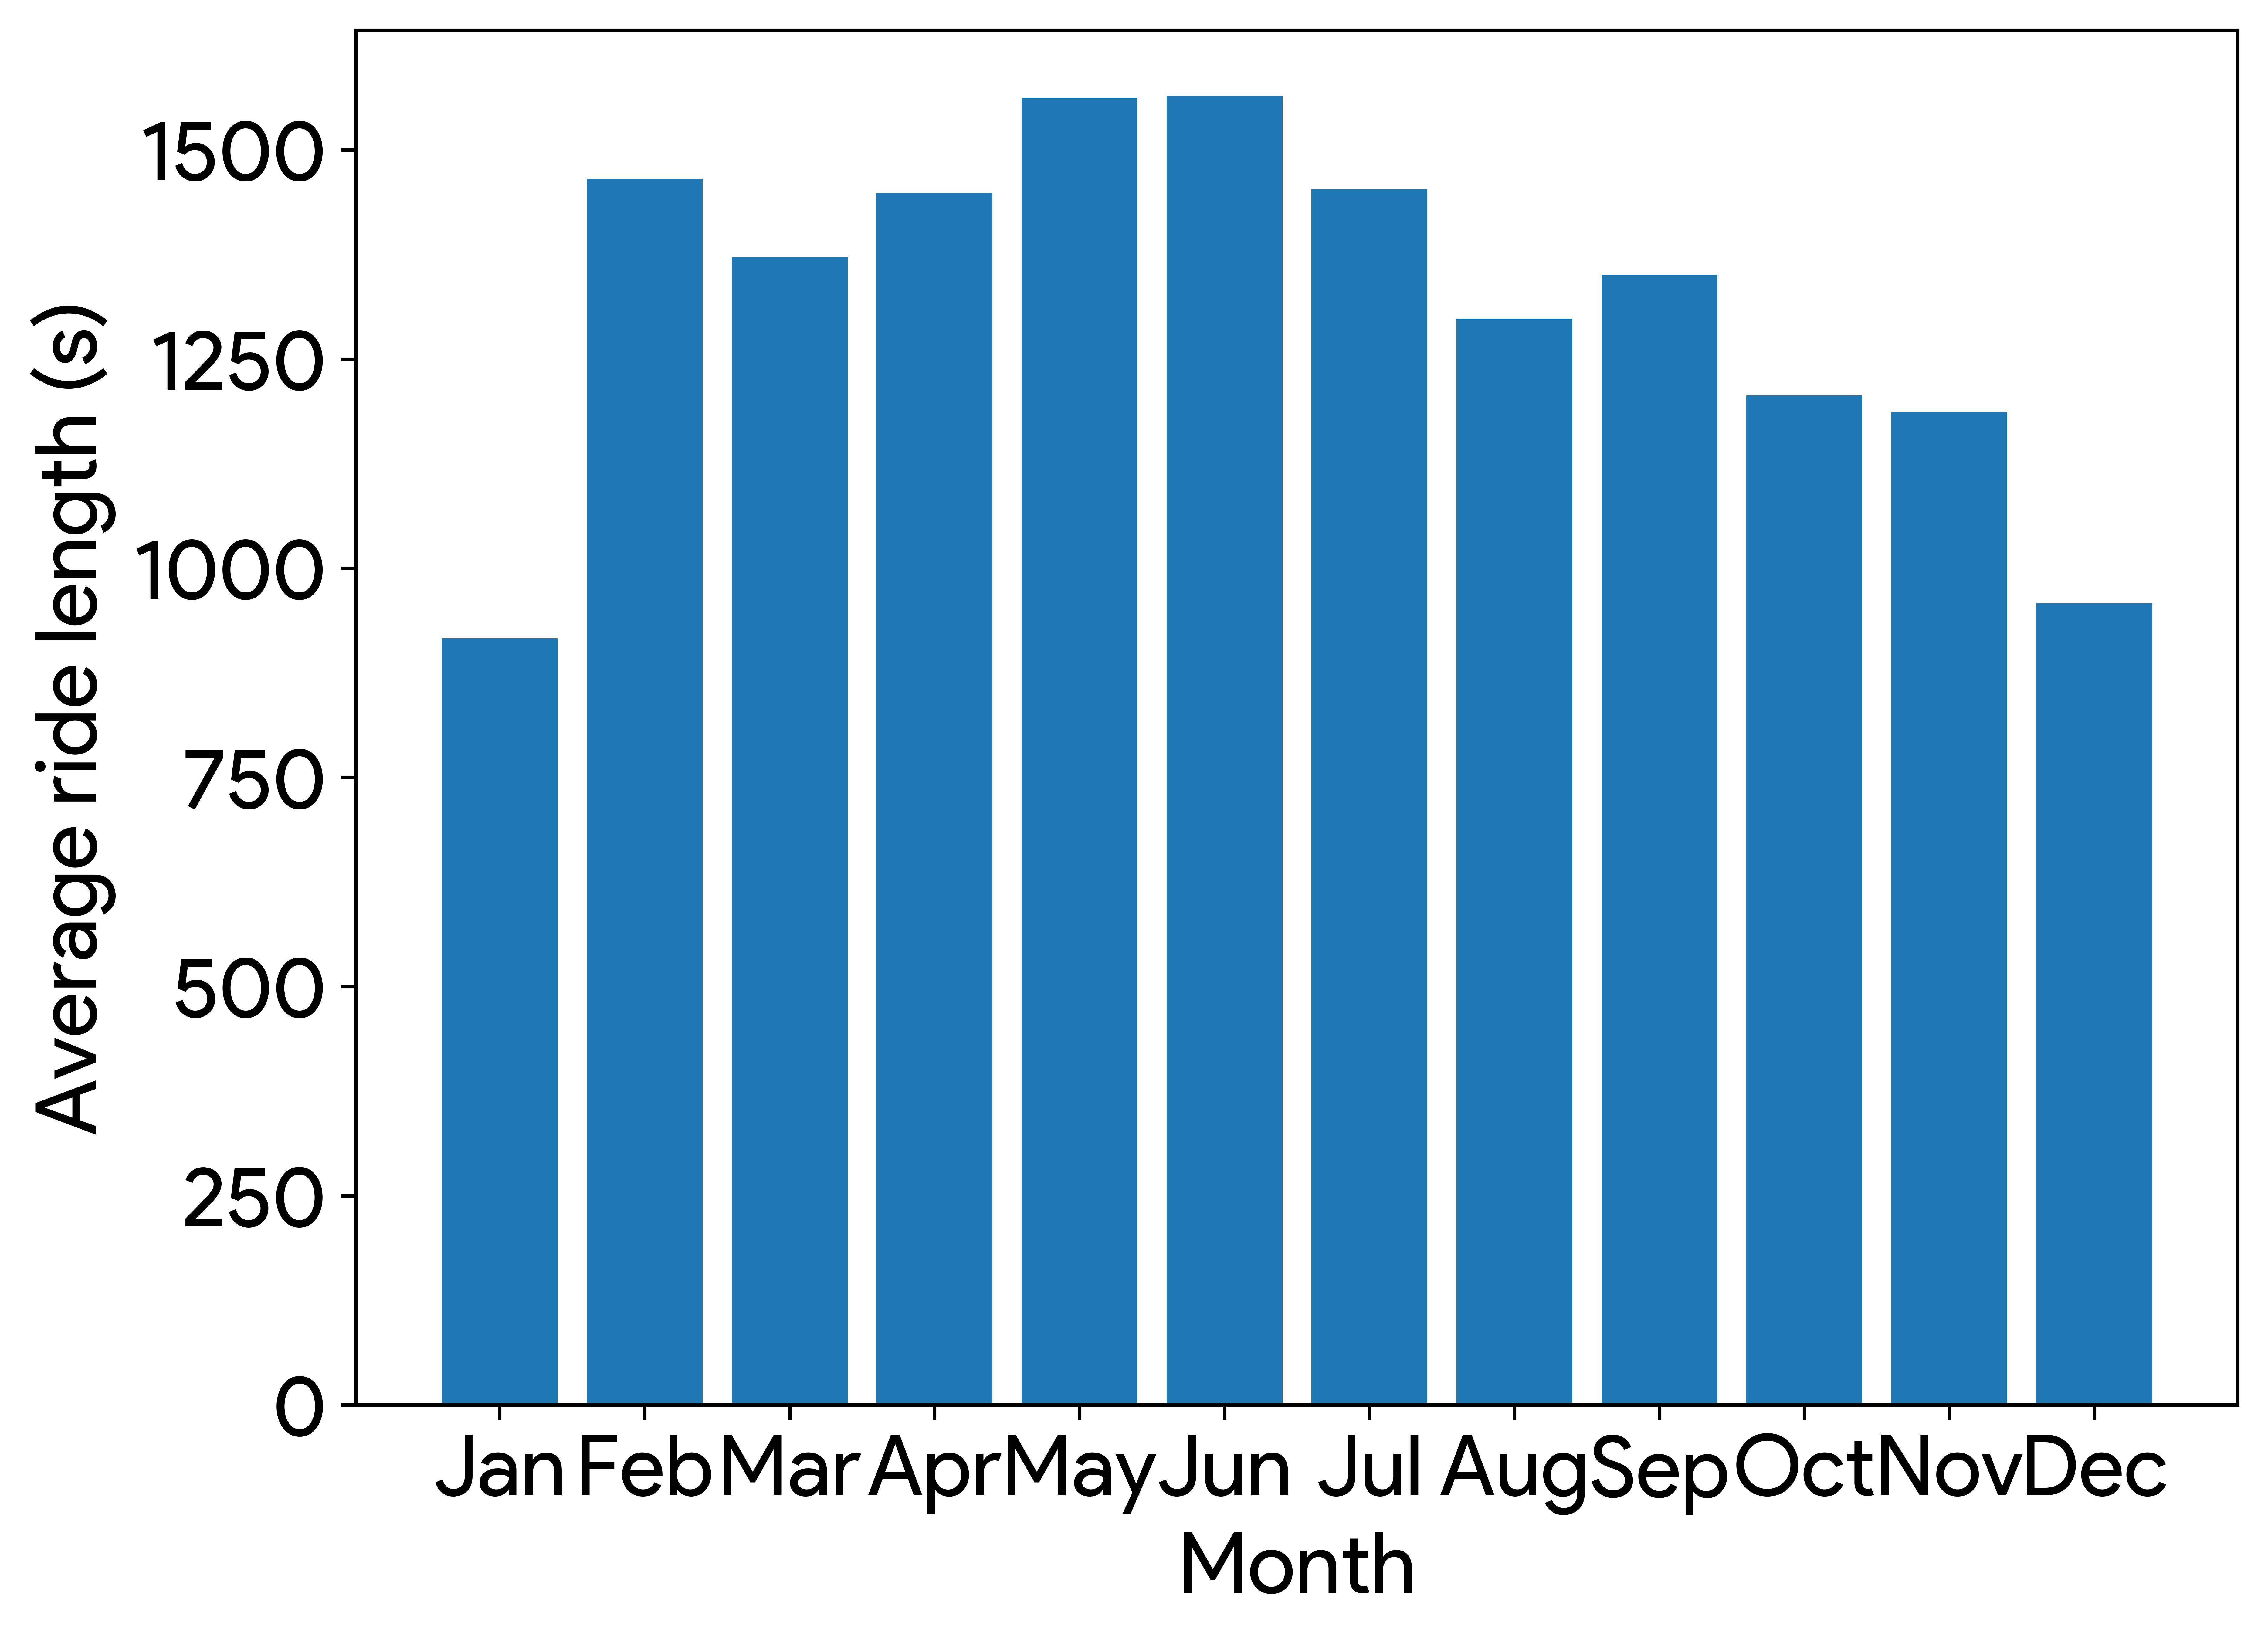
\includegraphics[width=\textwidth]{figs/ride_mean_month}
  \caption{Average ride length (in seconds) by month}
  \label{fig:ride_mean_month}
\end{figure}


We see clearly, from Fig~\ref{fig:ride_mean_month}, that the average ride duration drops off steadily in the colder months, with the months of December and January having the shortest average ride lengths. The transition from January to February is the sharpest uptick.

\iffalse
We see clearly, from Fig~\ref{fig:ride_mean_month}, that the average ride duration is significantly higher in the month of December, i.e., `holiday season.' While this may be due to any one (or multiple) of a number of possible reasons, what is true irrespective of the reason is that Cyclistic customers use the bike share service a lot during the holiday season. \textbf{So, something worth considering for the marketing team is to invest in advertising during the months leading up to the holiday season, and maybe even in the weeks leading up to other popular holidays like Thanksgiving, or Halloween.}
\fi

Next, we look at the variation of maximum ride length by month, as shown in Fig~\ref{fig:ride_max_month} below.

\begin{figure}[h]
  \centering
  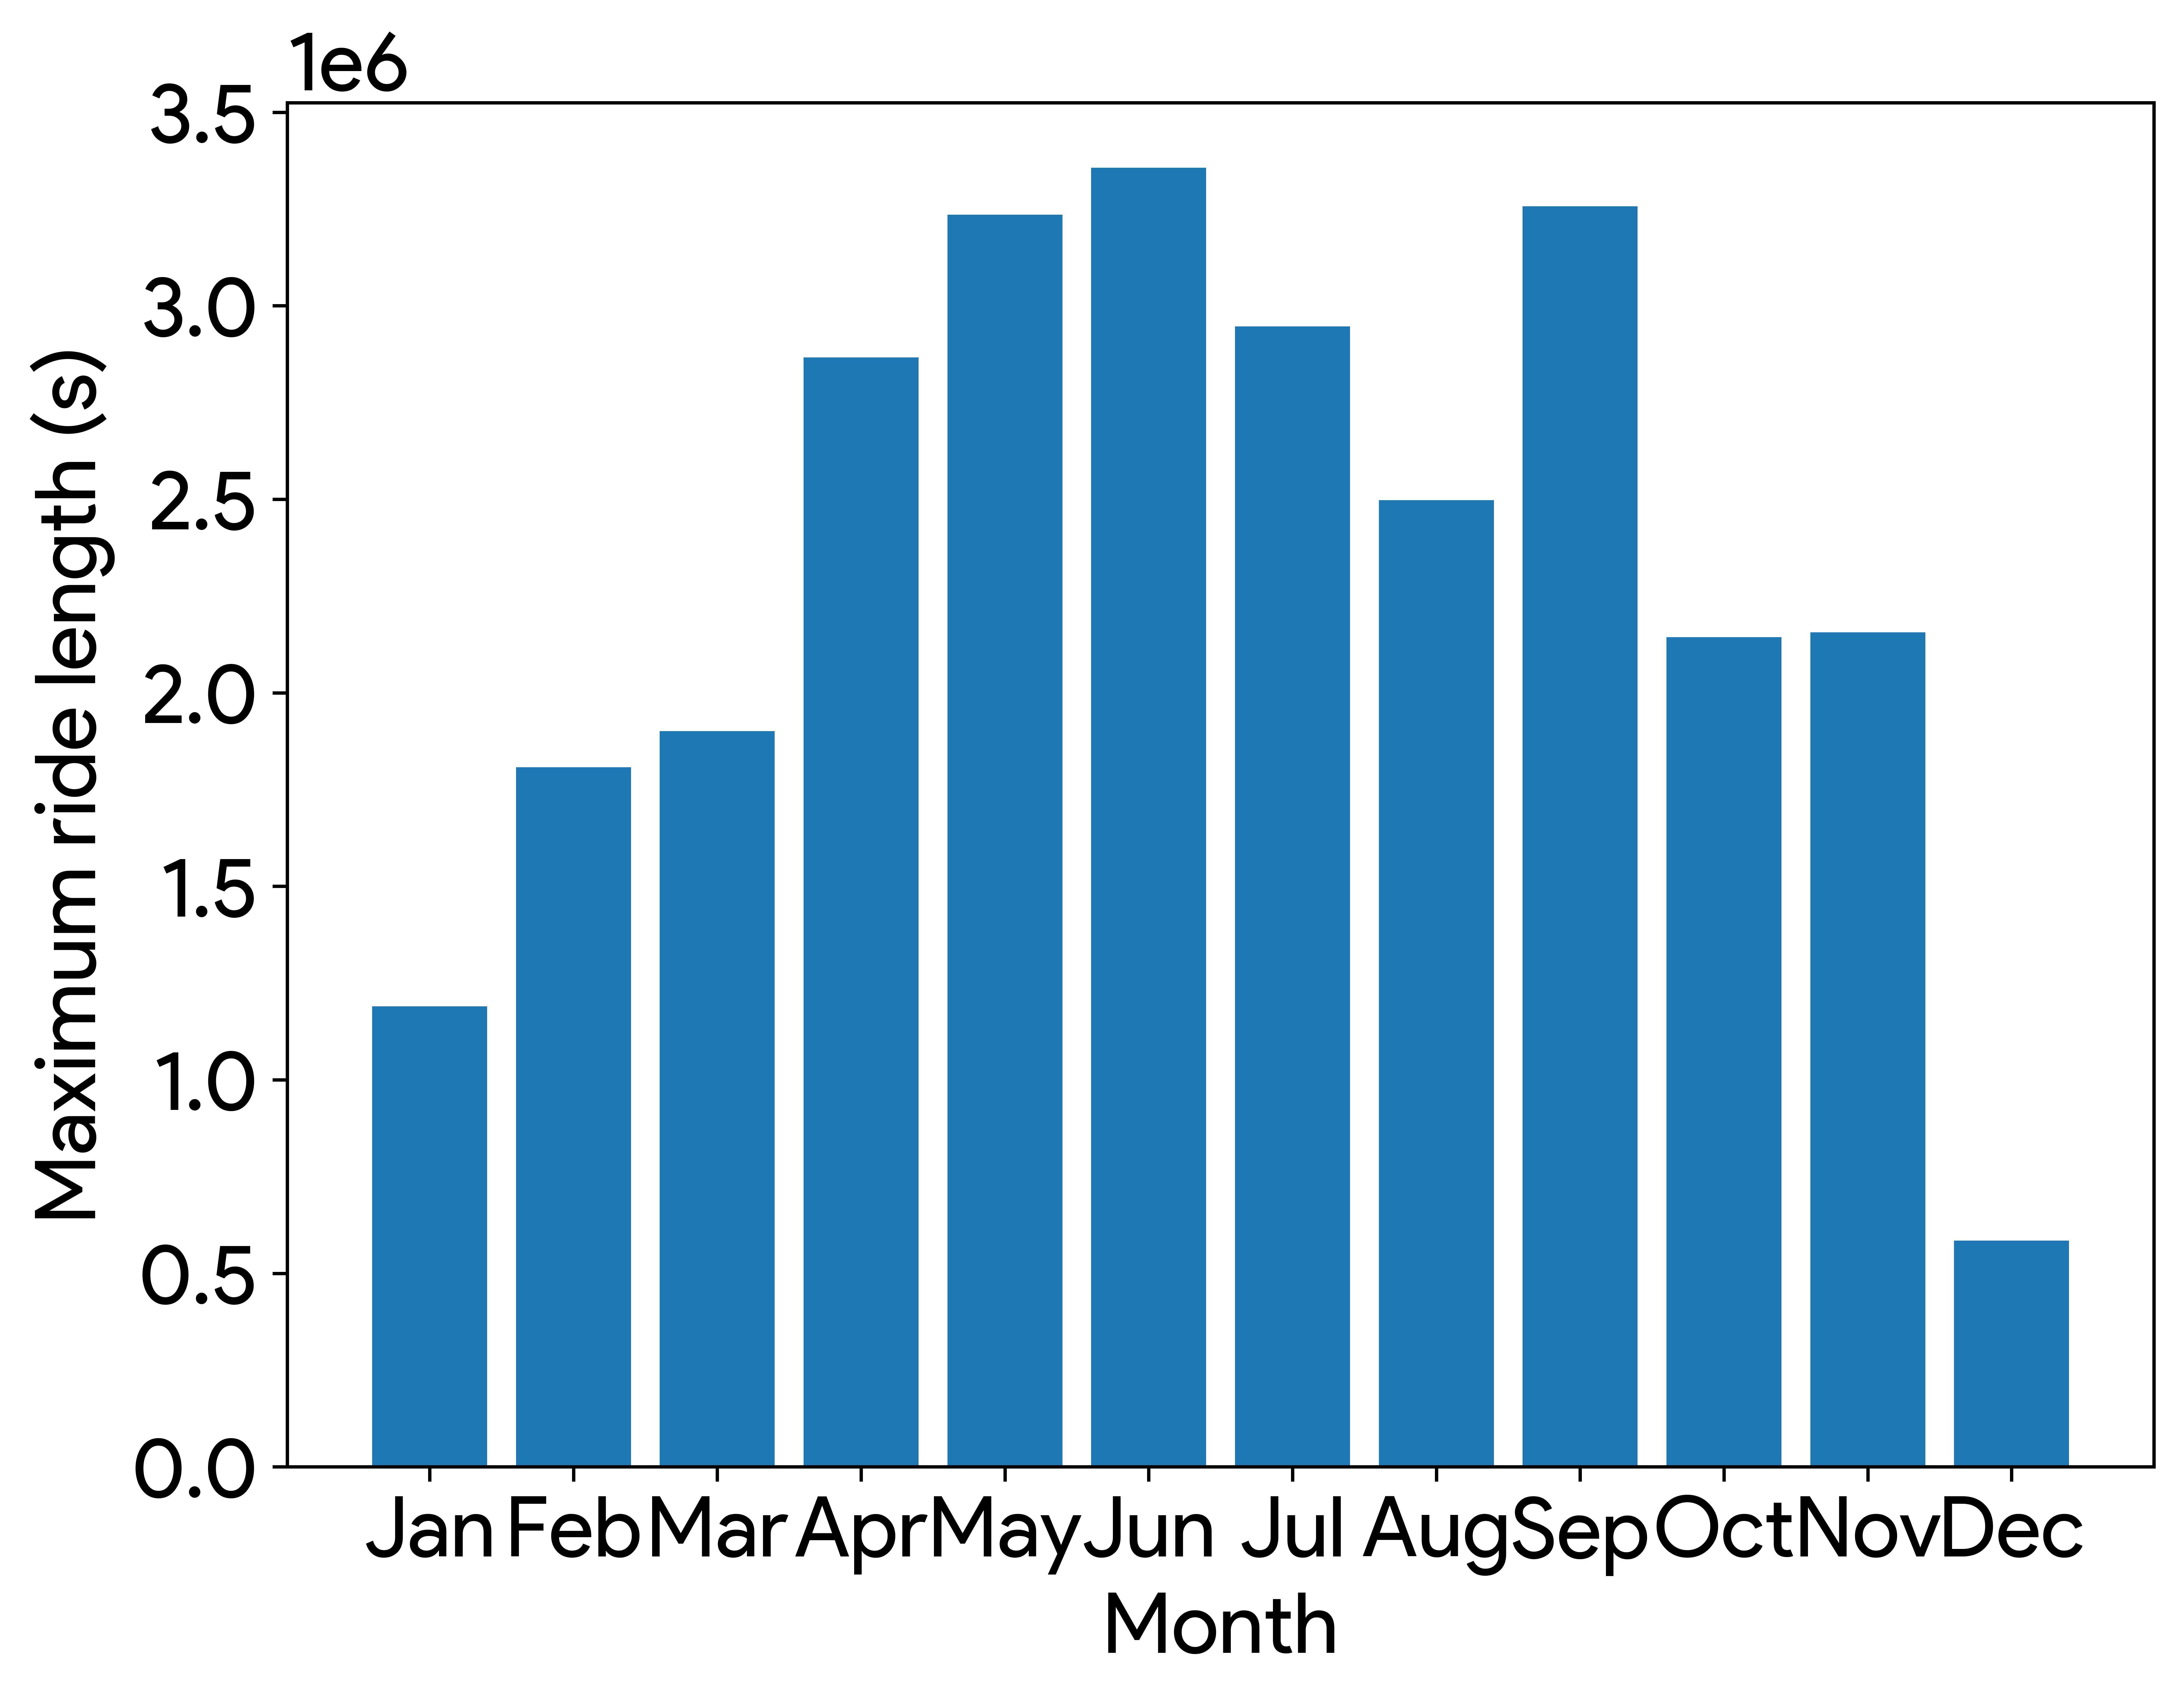
\includegraphics[width=\textwidth]{figs/ride_max_month}
  \caption{Maximum ride length (in seconds) by month}
  \label{fig:ride_max_month}
\end{figure}


We see, from Fig~\ref{fig:ride_max_month}, that the longest rides occur during the summer months, i.e., April to July. This seems a bit intuitive as people tend to spend longer amounts of time doing outdoor activities during the summer months when the weather conditions are more pleasant. \textbf{For the marketing team, we would like to suggest targeting people with more active lifestyles, and specifically, advertise to them during the SPring months leading up to the summer, so that when summer comes around and people are planning their activities, they would be more likely to consider using Cyclistic for their bike-share needs.} In addition, we also see a sharp increase again in the month of September. We could speculate this to have something to do with the beginning of the Fall semester, and students using the bike-share service for longer trips to get to their classes and back. So, advertising Cyclistic's services to students (or to-be-students) is something that could be worth exploring. But a reminder that this specific insight is just and educated guess, since the spike in maximum ride length in the month of September could potentially be due to several other reasons.

\iffalse
We see, from Fig~\ref{fig:ride_max_month}, that the longest rides occur during the summer months, i.e., April to July. This seems a bit intuitive as people tend to spend longer amounts of time doing outdoor activities during the summer months when the weather conditions are more pleasant. \textbf{For the marketing team, we would like to suggest targeting people with more active lifestyles, and specifically, advertise to them during the Spring months leading up to the summer, so that when summer comes around and people are planning their activities, they would be more likely to consider using Cyclistic for their bike-share needs.} In addition, we also see a sharp increase again in the month of September. We could speculate this to have something to do with the beginning of the Fall semester, and students using the bike-share service for longer trips to get to their classes and back. So, advertising Cyclistic's services to students (or to-be students) is something that could be worth exploring. But a reminder that this specific insight is just an educated guess, since the spike in maximum ride length in the month of September could potentially be due to several other reasons.
\fi



Next, we look at the average ride length as it changes by month, but showing `casual' users of the service and annual members separately, as shown in Fig~\ref{fig:ride_mem_month}.

\begin{figure}
  \centering
  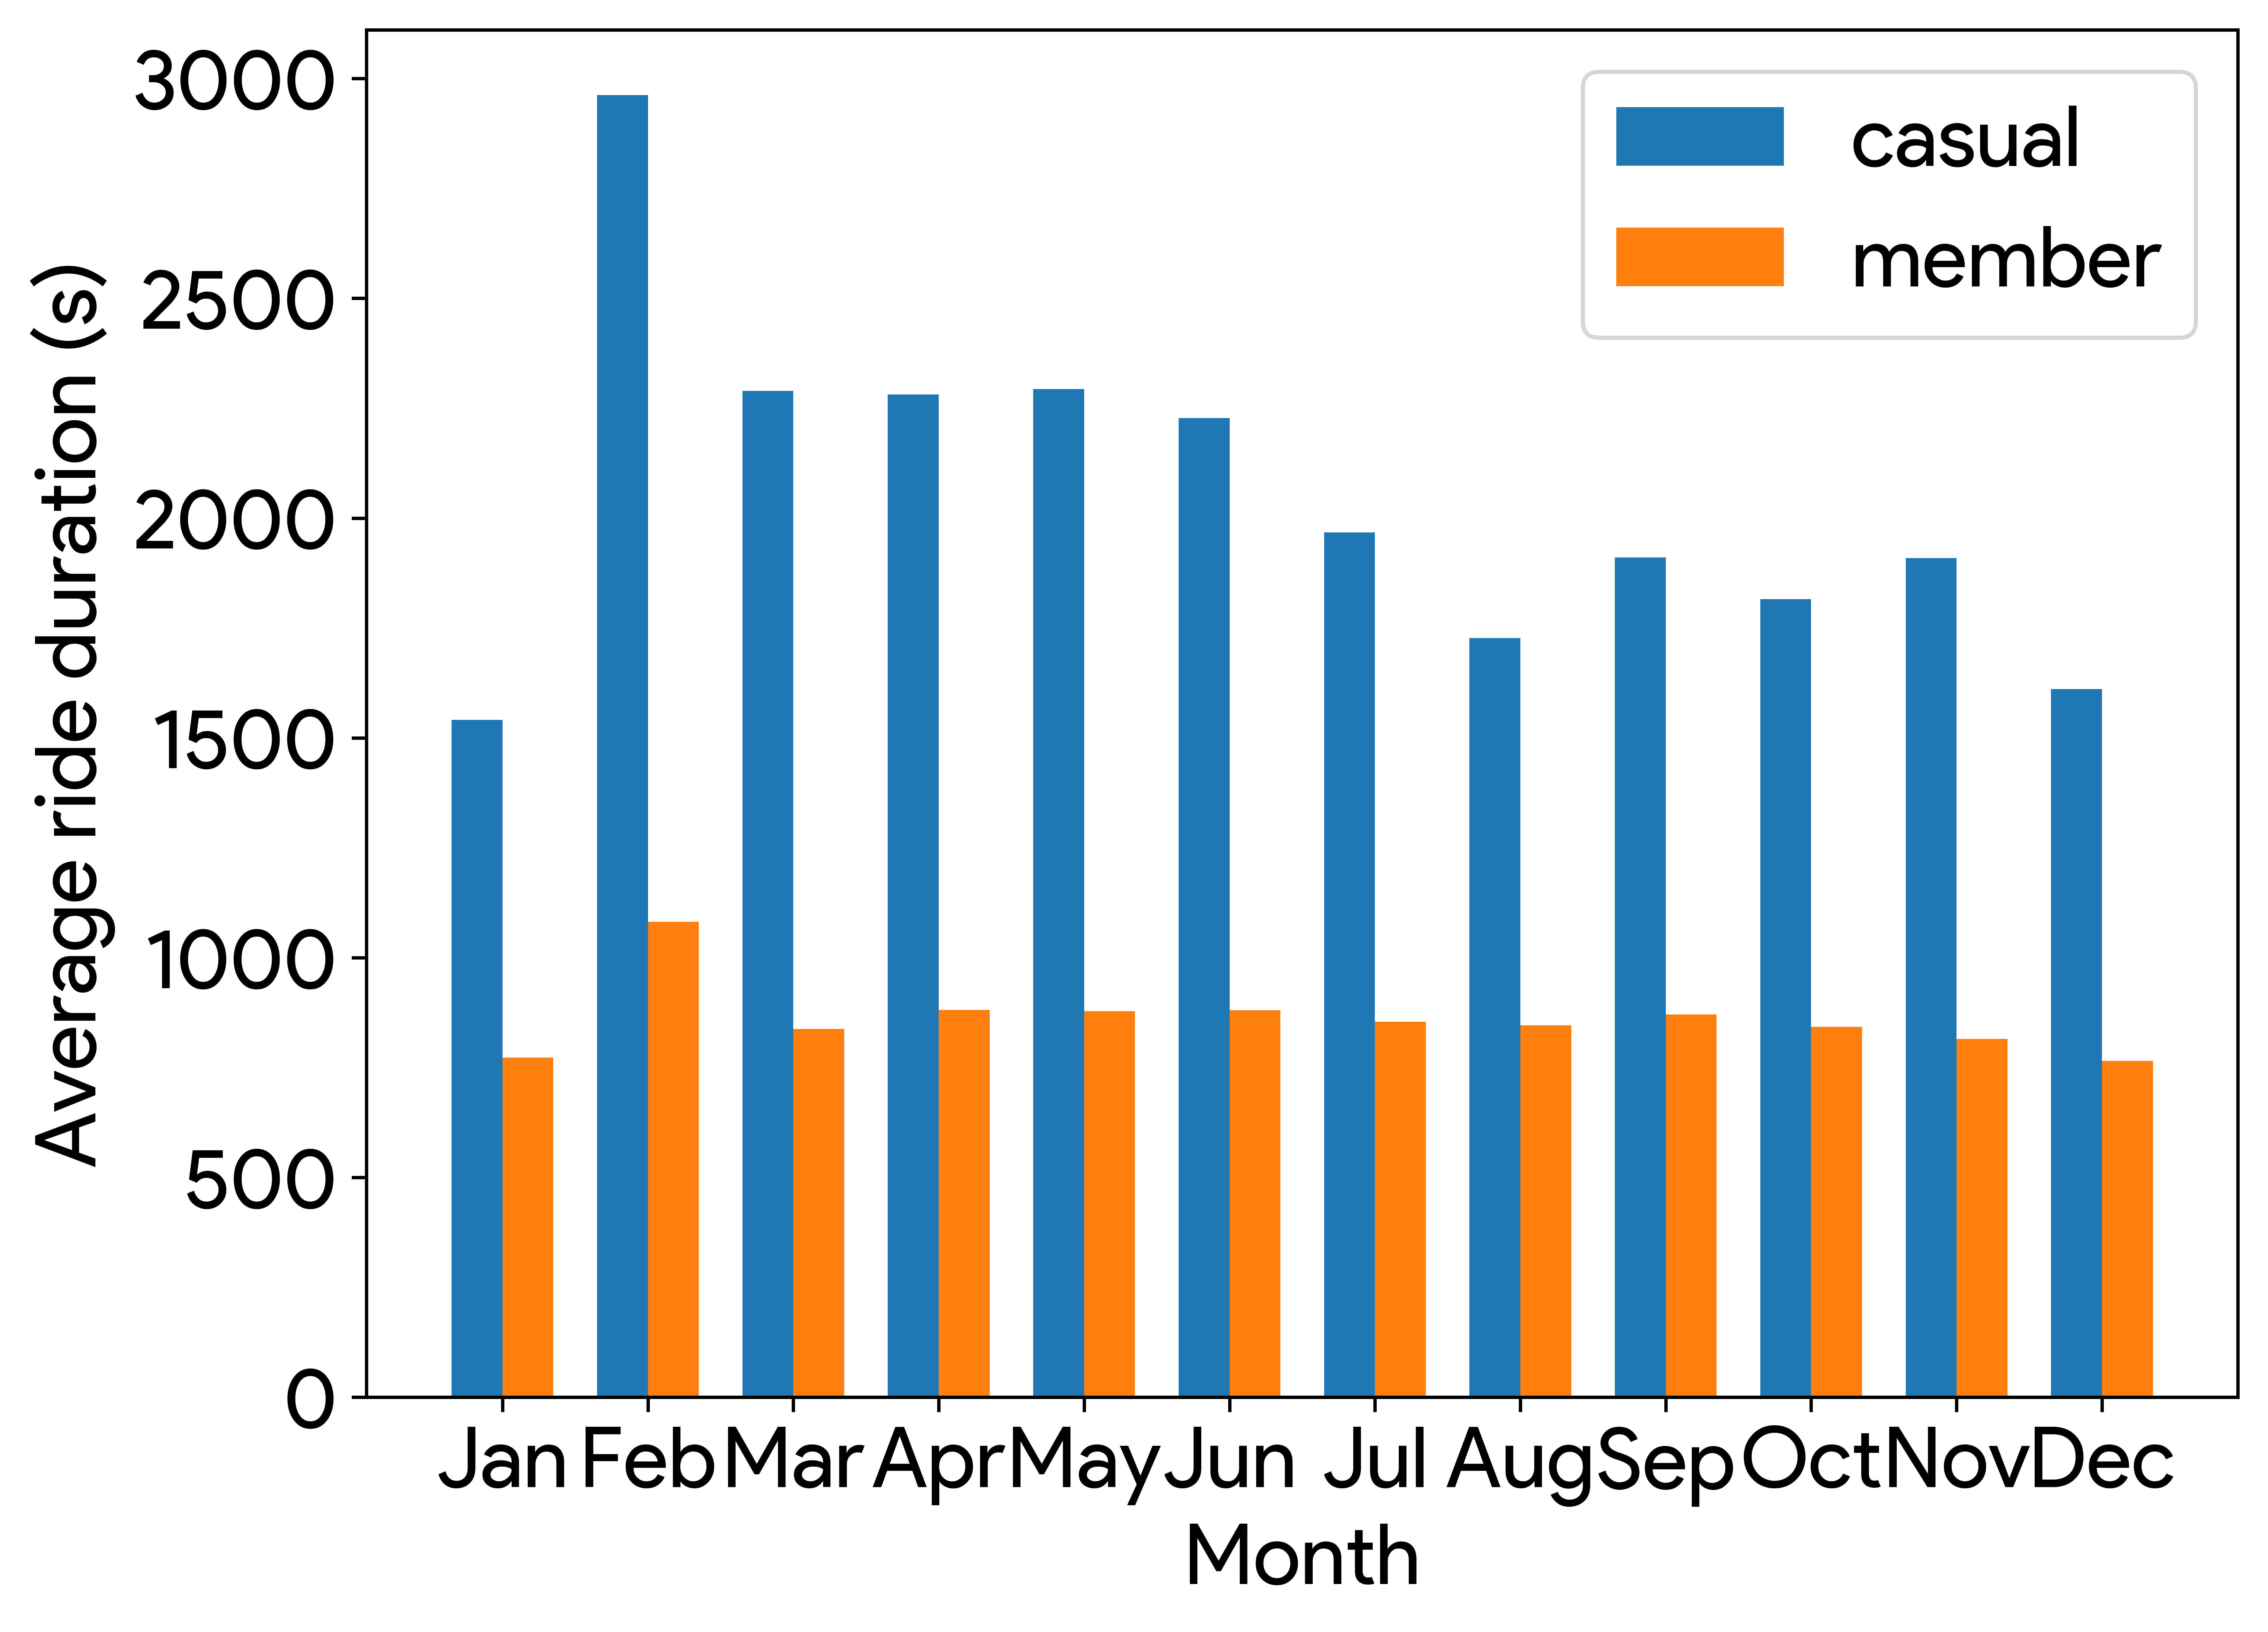
\includegraphics[width=\textwidth]{figs/ride_mem_month}
  \caption{Average ride length of annual members compared to `casual' users of Cyclistic's bike-share service by month}
  \label{fig:ride_mem_month}
\end{figure}


\textbf{We see, from Fig~\ref{fig:ride_mem_month} that casual users of Cyclistic's bike-share service take consistently longer rides than annual members, which is encouraging, since there are potentially cost-savings to be had for the casual users that could make for a very attractive marketing message}. Another thing worth noting is that the average ride length for annual members seems very consistent throughout the year, with the exception of the month of December. This seems to suggest that the people who have subscribed to the annual membership tend to use it in a consistent, repetitive manner, as opposed to the `casual' users of the service, where we see more of a variation in their average ride length through the year.

Finally, we would like to address the fact that the average ride length of `casual' users and annual members alike drops off drastically in the month of January. While this could probably be at least partially attributed to weather conditions, we note that the month of February, while still having similar `less pleasant' weather conditions, shows the second-highest average ride lengths (after the month of December). This likely suggests that January usage of the bike-share service has potential for improvement. \textbf{What this means for the marketing team is that they could probably offer some attractive membership deals/offers for the month of January}. Especially since the month of December already has the longest ride durations, some attractive offers (for the month of January) could be advertised to customers during the month of December, which might encourage them to use the bike-share service more. This could then potentially lead to more `casual' customers being converted to annual members.


\section{Share}

This document is designed to serve the purpose of sharing the insights that we have found from analyzing this dataset. The visualizations and the claims outlined here are meant to serve as an intriguing and engaging narrative of the insights that we have gleaned from this publicly available dataset, for the purpose of providing actionable directives for the Cyclistic marketing team.

\section{Act}

Based on the bike-share data spanning the last year, here are some of the high-level recommendations we have gathered for the marketing team at Cyclistic
\begin{itemize}
%\item We recommend the marketing team to consider investing in advertising heavily during the months leading up to the holiday season, and maybe even in the weeks leading up to other popular holidays like Thanksgiving, or Halloween.
\item We would like to suggest that the marketing team target advertising towards people with more active lifestyles, and specifically, advertise to them during the Spring months leading up to the summer, so that when summer comes around and people are planning their outdoor activities, they would be more likely to consider using Cyclistic for their bike-share needs.
\item Casual users of Cyclistic's bike-share service take consistently longer rides than annual members, which is encouraging, since there are potentially cost-savings to be had for the casual users that could make for a very attractive marketing message to propose that they become paid members of the service.
  \item Seeing the low ridership during the month of January, we suggest that the marketing team consider offer some attractive membership deals/offers for the month of January. Especially since the month of December already has the longest ride durations, some attractive offers (for the month of January) could be advertised to customers during the month of December, which might encourage them to use the bike-share service more. This could then potentially lead to more `casual' customers being converted to annual members.
\end{itemize}


\end{document}
